\subsection{Data in electrophysiology (M/EEG)}\label{data_in_electrophysiology}

Electrophysiology refers to a branch of physiology that study the electrical and electrochemical phenomena that occur in the cells or tissues of living organisms and, in particular, in neurons and muscle fibres.
In neuroscience, we are particularly interested in the electrical activity of the neurons and especially in the emission of post-synaptic potentials (PSP).
In a neuron, PSP are nerve influx along the axon consecutive to ion exchange at the synapse level, as shown in Figure~\ref{fig:post_synaptic_potentials}, which change the polarity of the cell membrane.
As moving charges on a wire induces an electo-magnetic field, a group of neurons in the gray matter\footnote{More precisely, the pyramidal cells in the cortex, that constitute approximately \SI{80}{\percent} of the neurons of the cortex.}, the upper part of the brain that is composed essentially of the cell bodies and the dendritic tree of neurons, form a current generator\footnote{Alexandre \textsc{Gramfort}, \textit{ Functional Brain Imaging with MEG, EEG and sEEG}, Université Paris-Saclay, MEEG course, \url{http://bit.ly/meeg_course}} that produces an electrical and a magnetic field.

\begin{figure}[h]
    \centering
    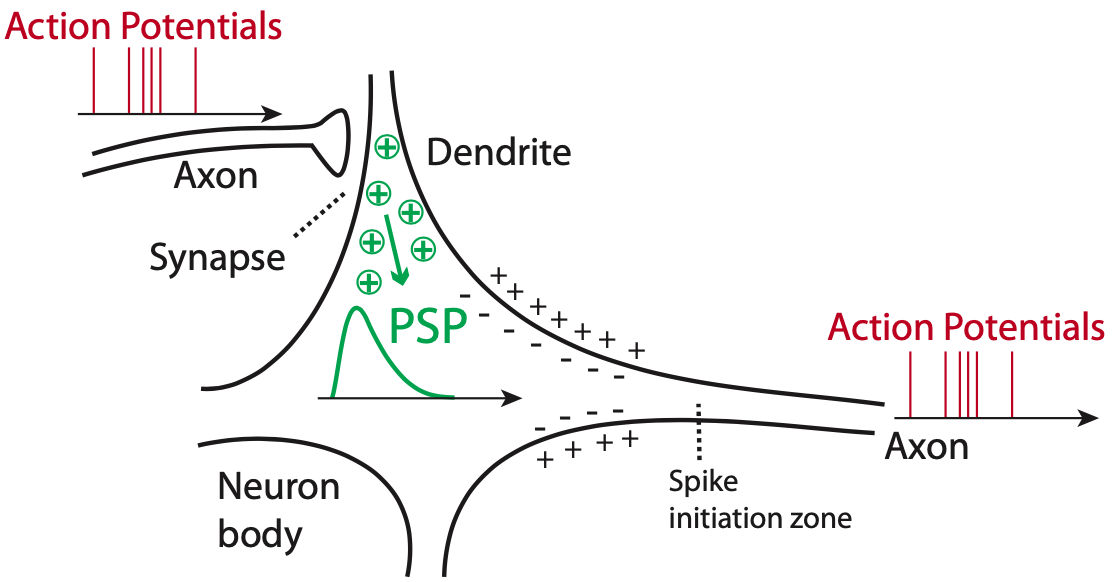
\includegraphics[scale=0.25]{pics/post-synaptic_potentials.png}
    \caption{Post-synaptic potentials in a neuron, consecutive to ion exchange}
    \source{A. \textsc{Gramfort}, MEEG course}
    \label{fig:post_synaptic_potentials}
\end{figure}

Two methods are used to capture both the electrical and the magnetic field, respectively the electroencephalography (EEG) that captures differences in electric potential at the scalp, and the magnetoencephalography (MEG) that captures magnetic flux density outside the head, as shown in Figure~\ref{fig:meeg_recordings}.
Both method record synchronised neural activity at a very high temporal resolution, about the millisecond\footnote{Sampling is often between \num{250} and \SI{1000}{\hertz}.}, and have the advantage of being non-invasive, unlike ectrocorticography (ECoG) that uses electrodes placed directly on the exposed surface of the brain.
Note that a large number of simultaneously active neurons, about \num{50000}, are needed to generate a measurable M/EEG signal\footnote{Saskia \textsc{Helbling}, \textit{What are we measuring with M/EEG?}, Goethe University Frankfurt, SPM course, May 2014}.

\begin{figure}
    \centering
    \begin{subfigure}[h]{0.45\textwidth}
        \centering
        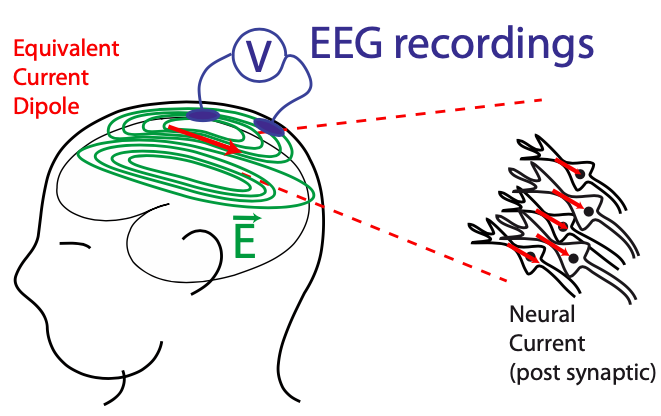
\includegraphics[width=0.9\textwidth]{pics/eeg_recordings.png}
        \caption{EEG recordings}
        \label{fig:eeg_recordings}
    \end{subfigure}
    \hfill
    \begin{subfigure}[h]{0.45\textwidth}
        \centering
        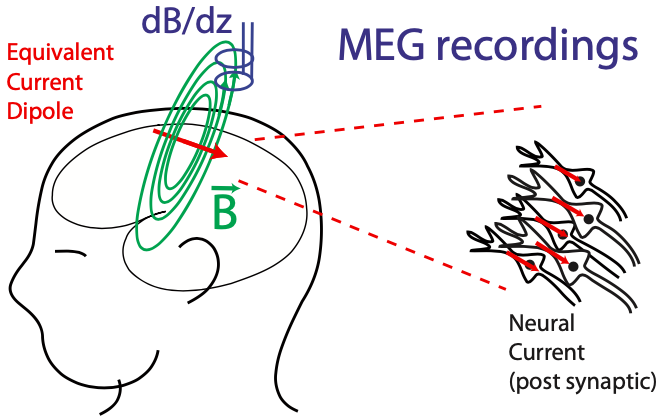
\includegraphics[width=0.9\textwidth]{pics/meg_recordings.png}
        \caption{MEG recordings}
        \label{fig:meg_recordings}
    \end{subfigure}
    \caption{Recordings of the electrical field (a) and the magnetic field (b).}
    \source{A. \textsc{Gramfort}, MEEG course}
    \label{fig:meeg_recordings}
\end{figure}

This high temporal resolution is what makes MEG and EEG attractive for the functional study of the brain.
The spatial resolution, on the contrary, is rather poor as only a few hundred simultaneous data positions can be acquired simultaneously (about \numrange{300}{400} sensors for MEG and up to \num{256} electrodes for EEG).
With appropriate models and methods, localisation of activity from MEG and EEG is nevertheless possible\footnote{\href{https://team.inria.fr/athena/fr/megeeg-vs-other-functional-brain-imaging-modalities/}{Inria: MEG/EEG vs. other functional brain imaging modalities}}.
This is what is called the \textit{inverse problem}, whose objective is to determine the current generators that produced the M/EEG measurements, as opposed to the \textit{forward problem} whose objective is to predict the M/EEG surface signal to current dipoles in the brain.

Finaly, note that neural activity recorded via M/EEG measurements is fundamental to modern experimental neuroscience and in our understanding of human cognitive processes and certain pathologies, thereby motivating the development of computational tools for learning such signals from data.
Such recordings consist of dozens to hundreds of simultaneously recorded signals, for duration going from minutes to hour \citep{jas2017learning, dupre2018multivariate}.

In this report we will mainly focus on the data recorded via MEG obtained in the course of experiments in which subjects are exposed to external stimuli.
A more comprehensive presentation of the data we work with is done in the Section~\ref{res_real_data}.
In Python, M/EEG data are easily manipulable thanks to the \href{https://mne.tools/stable/index.html}{\texttt{MNE} package} \citep{gramfort2013meg}.
